%=======================02-713 LaTeX template, following the 15-210 template==================
%
% You don't need to use LaTeX or this template, but you must turn your homework in as
% a typeset PDF somehow.
%
% How to use:
%    1. Update your information in section "A" below
%    2. Write your answers in section "B" below. Precede answers for all 
%       parts of a question with the command "\question{n}{desc}" where n is
%       the question number and "desc" is a short, one-line description of 
%       the problem. There is no need to restate the problem.
%    3. If a question has multiple parts, precede the answer to part x with the
%       command "\part{x}".
%    4. If a problem asks you to design an algorithm, use the commands
%       \algorithm, \correctness, \runtime to precede your discussion of the 
%       description of the algorithm, its correctness, and its running time, respectively.
%    5. You can include graphics by using the command \includegraphics{FILENAME}
%
\documentclass[11pt]{article}
\usepackage{amsmath,amssymb,amsthm}
\usepackage{graphicx}
\usepackage[margin=1in]{geometry}
\usepackage{fancyhdr}
\usepackage{tikz}
\usetikzlibrary{automata, positioning, arrows}
% \tikzset{
% 	->, % makes the edges directed
% 	>=stealth’, % makes the arrow heads bold
% 	node distance=3cm, % specifies the minimum distance between two nodes. Change if necessary.
% 	every state/.style={thick, fill=gray!10}, % sets the properties for each ’state’ node
% 	initial text=$ $, % sets the text that appears on the start arrow
% }
\newtheorem{theorem}{Theorem}
\newtheorem{conjecture}{Conjecture}
\setlength{\parindent}{0pt}
\setlength{\parskip}{5pt plus 1pt}
\setlength{\headheight}{13.6pt}
\newcommand\question[2]{\vspace{.25in}\hrule\textbf{#1}: #2\vspace{.5em}\hrule\vspace{.10in}}
\renewcommand\part[1]{\vspace{.10in}(#1)\par}
\newcommand\algorithm{\vspace{.10in}\textbf{Algorithm: }}
\newcommand\correctness{\vspace{.10in}\textbf{Correctness: }}
\newcommand\runtime{\vspace{.10in}\textbf{Running time: }}
\newcommand{\R}{\mathbb{R}}
\newcommand{\N}{\mathbb{N}}
\newcommand{\Z}{\mathbb{Z}}
\pagestyle{fancyplain}
\lhead{\textbf{\NAME}}
\chead{\textbf{{\COURSE} Homework \HWNUM}}
\rhead{\today}
\begin{document}\raggedright
%Section A==============Change the values below to match your information==================
\newcommand\NAME{Eric Altenburg}  % your name
\newcommand\COURSE{MA-240}
\newcommand\HWNUM{9 Corrections}              % the homework number
%Section B==============Put your answers to the questions below here=======================

% no need to restate the problem --- the graders know which problem is which,
% but replacing "The First Problem" with a short phrase will help you remember
% which problem this is when you read over your homeworks to study.

\textbf{Pledge:} \textit{I pledge my honor that I have abided by the Stevens Honor System.} -Eric Altenburg

\question{1}{The \textit{complete graph} on $n$ vertices, denoted $K_n$, is the graph with $ n \ge 1$ vertices such that each pair of distinct vertices is connected with a single edge. Prove that $K_n$ has an Euler circuit if and only if $n$ is odd. (You may assume results about Euler circuits that we proved in class.)}

\begin{proof}
	$(\Longrightarrow)$ If the complete graph $K_n$ with $n$ vertices has an Euler circuit, then $n$ must be odd. We know that a graph only has an Euler circuit if every vertex has an even degree. Additionally, in a complete graph with $n$ vertices every vertex has a degree of $n-1$. With this, we know $K_n$ has an Euler circuit which means every vertex has an even degree, and since it is a complete graph, every vertex has degree $n-1$. From this we can deduce that $n$ must be odd because $n-1$ is even.
	\newline
	$(\Longleftarrow)$ If $n$ is odd, then the complete graph $K_n$ with $n$ vertices has an Euler circuit. Using the same characteristics of complete graphs and Euler circuits, each of $K_n$'s vertices must have a degree of $n-1$. Because $n$ is odd, then that must mean $n-1$ is even. This means each vertex has an even degree, therefore, $K_n$ must have an Euler circuit.
\end{proof}

\question{2}{A graph $G=(V,E)$ is \textit{bipartite} if there exists a bipartition (a partition into two subsets) $V=V_1\sqcup V_2$ of its vertex set such that every edge in $E$ connects a vertex in $V_1$ to a vertex in $V_2$. Prove that a graph is bipartite if and only if it has no odd-length circuits.}

\begin{proof}
	$(\Longrightarrow)$ If a graph $G=(V,E)$ is bipartite, then it has no odd-length circuits. Then $G$'s vertices $V=V_1 \sqcup V_2$ with an edge $E$ connecting a vertex from $V_1$ to $V_2$. This means that while traversing the circuit, each edge will always lead from $V_1$ to $V_2$ or $V_2$ to $V_1$. Because a circuit requires that you end at the same vertex you start at, when traversing from the set $V_1$ to $V_2$ back to $V_1$, or $V_2$ to $V_1$ back to $V_2$, this will always be 2 moves. Going to the opposite set and back will occur $m$ times until you end at the same vertex you started out at, and so the length will be $2\cdot m$ which means the circuit will always have an even length.

	$(\Longleftarrow)$ If there are no odd-length circuits in a graph $G=(V,E)$, then $G$ is bipartite. Assume that every circuit in $G$ is of even-length. Now, choose any vertex in $G$ to be $v_0$, and any other vertex in $G$ to be $u$. For any $u$ in the same component $C_0$ as $v_0$ in $G$ we can define the length of the shortest path from $v_0$ to $u$ to be $d(v_0,u)$. Using this new function, starting at $v_0$ in $C_0$ label it as $EVEN$, and for all other vertices in $C_0$ represented as $u$, if $d(v_0, u)$ returns a path that is of even length, then label $u$ as $EVEN$, else if it is ODD, then label $u$ as $ODD$. Repeat this for every component in $G$. 

	Now we have a graph where every vertex is labeled as either $EVEN$ or $ODD$; these two labels will form the two sets that each vertex will belong to for the bipartite graph. If there is any edge that connects two vertices with the same label (i.e. $ODD$ to $ODD$ or $EVEN$ to $EVEN$), then there must be a cycle with an odd length. 

	To show this is true, suppose the first vertex is $v_1$ and the other is $v_2$. If both $v_1$ and $v_2$ have a label of $EVEN$, then they must have an even distance from $v_0$. If we take these two lengths and account for the edge that joins them, then for some $k$ we will get a cycle starting from $v_0$ of length $$EVEN+EVEN+1 = 2k + 2k + 1 = 2(2k)+1$$ which is an odd number. Additionally, if $v_1$ and $v_2$ were labeled as $ODD$ and accounting for the additional edge joining them, for some $k$ we get a cycle from $v_0$ that has the length $$ODD + ODD + 1 = (2k+1)+(2k+1)+1 = 2(2k+1)+1$$ which is an odd number as well. 

	Therefore, knowing now that the cycles would be of odd length, then this means there will be two vertices that belong to the same set and are directly connected with an edge making $G$ a non-bipartite graph. However, if this is not true and no like-labeled vertices are connected with an edge, then all cycles must be of even-length and so $G$ a bipartite graph such that $V=EVEN \sqcup ODD$.
\end{proof}

\question{3}{A \textit{bidirectional Euler circuit} is a circuit in which each edge is traveled exactly twice, once in each direction. Prove that every finite connected graph has a bidirectional Euler circuit.}

\begin{proof}
	Because a bidirectional Euler circuit uses every edge exactly twice, once in each direction, we can use this to split each edge of a graph to force an Euler circuit. If we know there is an Euler circuit, then we can traverse the reversal of such a circuit to satisfy the properties of a bidirectional Euler circuit. \\
	Suppose there is a finite connected graph $G$ where any number of its vertices has odd or even degrees. Initially, it is not known whether or not an Euler circuit exists in $G$ because it is possible that one or more vertices have an odd degree. However, because we need to have a circuit such that each edge is traversed exactly twice, once in each direction, we can then construct an equivalent graph $G^{\prime}$ that has all the same edges and vertices as $G$, but now every edge in $G^{\prime}$ connecting two vertices will be split into two. One will be used to traverse in one direction and the other will be used to traverse in the other; graphically, although these are now directed edges, because both are being used in combination, they still act as an undirected edge. To show this graphically, see Figure~\ref{initial_graph}.

	\begin{figure}[ht]
		\centering
		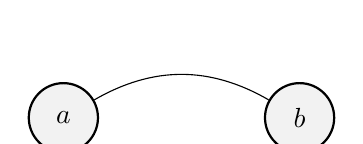
\begin{tikzpicture}[node distance=3cm, every state/.style={thick, fill=gray!10}, initial text=$ $, baseline={(0,0)}]
			\node[state] (left_node) {$a$};
			\node[state, right of=left_node] (right_node) {$b$};
			\draw (left_node) edge[bend left] (right_node);
		\end{tikzpicture}
		\quad $\equiv$ \quad
		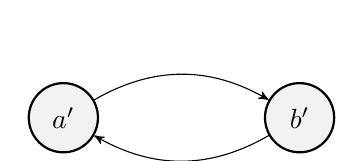
\begin{tikzpicture}[->, >=stealth', node distance=3cm, every state/.style={thick, fill=gray!10}, initial text=$ $,baseline={(0,0)}]
			\node[state] (left_node) {$a^{\prime}$};
			\node[state, right of=left_node] (right_node) {$b^{\prime}$};
			\draw 	(left_node) edge[bend left] (right_node)
					(right_node) edge[bend left] (left_node);
		\end{tikzpicture}
		\caption{(Left) Initial two vertices without the edge being split. (Right) Same two vertices but now the edge has been split to add an additional one to represent the bidirectional property.}
		\label{initial_graph}
	\end{figure}

	Adding a new edge to each pair of connected vertices in $G^{\prime}$ would then double the degree of each vertex making it such that each vertex will have an equal amount of in-degrees and out-degrees. From this, we can conclude that there must exist an Euler circuit in $G^{\prime}$, and traversing this path initially will ensure that each edge is traversed exactly once in one direction. Now, simply traverse the reversal of this new circuit making it so that each edge has now been traversed twice, once in each direction. Therefore, because $G^{\prime}$ is equivalent to $G$, this proves that every finite connected graph has a bidirectional Euler circuit.
\end{proof}















	
\end{document}